\documentclass{tuna-report}
\usepackage{codespace}
\usepackage{caption}
\usepackage{subcaption}
\usepackage{wrapfig}
\usepackage{graphicx}
\usepackage{array}
\usepackage[super]{nth}
\usepackage{longtable}
\usepackage{listings} % For code snippets 

% \usepackage[colorlinks]{hyperref}
%\usepackage[printonlyused,withpage]{acronym} %abbreviations
\usepackage{acro}
% Sub-preambles
% https://github.com/MartinScharrer/standalone

% Encodings
\usepackage{gensymb,textcomp}

% Better tables
% Wide tables go to https://tex.stackexchange.com/q/332902
\usepackage{array,multicol,multirow,siunitx,tabularx}

% Better enum
\usepackage{enumitem}

% Graphics
\usepackage{caption,float}

% Allow setting >max< width of figure
% 'export' allows adjustbox keys in \includegraphics
% For demonstration purposes, remove in production
\usepackage[export]{adjustbox}

% For demonstration purposes, remove in production
\usepackage{mwe}


% Configurations
\newcounter{memberrowno}
\setcounter{memberrowno}{0}
\setcounter{tocdepth}{5}
\reportlayout%

% Override (some) default values
\ocoursename{Bachelor Thesis in Computer Science}
\title{Practical Training Report}


% ================== Custom commands
\newcommand*\mean[1]{\bar{#1}}

% Set up the command for a blank page
\usepackage{afterpage}

\newcommand\blankpage{%
    \null
    \
    \vfil
    \hfil (Intentionally left blank) \hfil
    \vfil
    \thispagestyle{empty}%
    % \addtocounter{page}{-1}%
    \newpage}
    
   
% ========================================

\graphicspath{ {graphics/} }

% Disable hypcap for specific captions
\captionsetup[figure]{hypcap=false}

% =================DECLARE ACRONYMS=======================
\DeclareAcronym{usa}{
	short=USA,
	long=United States of America,
}
\DeclareAcronym{eu}{
	short=EU,
	long=European Union,
}
\DeclareAcronym{ussr}{
	short=USSR,
	long=Union of Soviet Socialist Republics,
}

% ================ STYLE FOR JS PROGRAMMING LANGUAGE ===============
\usepackage{xcolor}

\definecolor{codegreen}{rgb}{0,0.6,0}
\definecolor{codegray}{rgb}{0.5,0.5,0.5}
\definecolor{codepurple}{rgb}{0.58,0,0.82}
\definecolor{backcolour}{rgb}{0.95,0.95,0.92}
\definecolor{magenta}{rgb}{1,0,1} % Magenta for JavaScript keywords


% Define JavaScript as a language in listings
\lstdefinelanguage{JavaScript}{
	keywords={break, case, catch, continue, debugger, default, delete, do, else, finally, for, function, if, in, instanceof, new, return, switch, this, throw, try, typeof, var, let, const, while, with, yield, async, await, of},
	keywordstyle=\color{magenta}\bfseries, % Magenta for keywords
	ndkeywords={class, export, boolean, throw, implements, import, this},
	ndkeywordstyle=\color{magenta}, % Magenta for additional keywords
	identifierstyle=\color{black},  % Default color for variables
	sensitive=true,                 % Case-sensitive
	comment=[l]{//},                % Single-line comments
	morecomment=[s]{/*}{*/},        % Multi-line comments
	commentstyle=\color{codegreen}\ttfamily, % Comments in green
	stringstyle=\color{codepurple},          % Strings in purple
	morestring=[b]',                % Single quotes for strings
	morestring=[b]"                 % Double quotes for strings
}


\lstset{
	language=JavaScript,               % Set JavaScript as the language
	backgroundcolor=\color{backcolour},   
	commentstyle=\color{codegreen},
	keywordstyle=\color{magenta},
	numberstyle=\tiny\color{codegray},
	stringstyle=\color{codepurple},
	basicstyle=\ttfamily\footnotesize,
	breakatwhitespace=false,         
	breaklines=true,                 
	captionpos=b,                    
	keepspaces=true,                 
	numbers=left,                    
	numbersep=5pt,                  
	showspaces=false,                
	showstringspaces=false,
	showtabs=false,                  
	tabsize=2,
	frame=single
}

\renewcommand{\lstlistingname}{Code snippet}	% For lisitngs caption name
\renewcommand{\lstlistlistingname}{List of Code Snippets}	% For codes listing table title

% ========================= BEGIN DOCUMENT =======================
\begin{document}
	
\coverpage
\clearpage
\afterpage{\blankpage}
\centerline{\LARGE \textbf{Declarations}}

\vspace{10mm}

I hereby declare that this internship report is the result of my independent work undertaken following the completion of the internship program at Bosch Global Software Technologies Vietnam (BGSW Vietnam). The primary objective of this report is to meet the requirements of my academic curriculum. I affirm that all the data and interpretations provided in this document originate from my individual efforts during the internship period. It is imperative to emphasize that any viewpoints articulated in this report are entirely independent and do not reflect the official policies of the Vietnamese–German University and Bosch Global Software Technologies Vietnam (BGSW Vietnam).

% \vspace{90mm}
\vfill

\begin{tabular}{@{}p{3.5in}p{0.1in}p{1.5in}@{}}
  \hrulefill & & \hrulefill \\
  Vu Hoang Tuan Anh & & Date \\
  Program: Computer Science and Engineering & & \\ 
  FraUAS Student ID: 1403143 & & \\
  VGU Student ID: 18812 & & \\
  Intake: 2020 - 2024 & & \\
  Frankfurt University of Applied Sciences & & \\
  Vietnamese-German University & & \\
  % \centering
  % Some lengthy designation that makes the above-mentioned person feel 
  % special to everyone who reads this
\end{tabular}
\centerline{\LARGE \textbf{Supervisor Confirmation}}

\vspace{10mm}

The commencement of the internship was formally arranged through mutual agreement between the Vietnamese-German University and Bosch Global Software Technologies Vietnam (BGSW Vietnam). Additionally, Bosch’s endorsement, as evidenced by the signature, confirms my compliance with their established protocols, my thorough understanding of the assigned responsibilities, and the successful completion of all work tasks. Furthermore, the signatory has reviewed and agreed with the entirety of this report, which accurately and faithfully represents my internship experience at Bosch Global Software Technologies Vietnam (BGSW Vietnam).

% \vspace{130mm}
\vfill

\begin{tabular}{@{}p{3.5in}p{0.1in}p{1.5in}@{}}
  \hrulefill & & \hrulefill \\
    Mr. xxx xxx xxx & & Date \\
    %Technical project manager, delivery manager and% 
    Talent manager & & \\
    Bosch Global Software Technologies Vietnam & & \\
  % \centering
  % Some lengthy designation that makes the above-mentioned person feel 
  % special to everyone who reads this
\end{tabular}


%\printacronyms
%	\newpage
\listoffigures
	\newpage
\listoftables
	\newpage
\lstlistoflistings
	\newpage
	
\tableofcontents

% \newpage



\section{Acknowledgments}

% \begin{flushright}
%     Hello 
% \end{flushright}

First and foremost, I wish to convey my deepest gratitude to the distinguished faculty at the Vietnamese-German University and Frankfurt University of Applied Science. Their steadfast guidance and support have been pivotal in my academic and personal development throughout my four-year undergraduate studies. \\ \\
Secondly, I wish to express my sincere gratitude to Mr. Nguyen Son Giang, my esteemed manager, for his invaluable guidance and unwavering support throughout the duration of my academic pursuit. His mentorship has been instrumental in enabling me to explore and develop my skills in the domain of Web Development, while also fostering a deep and lasting interest in this field. \\ \\
Furthermore, I wish to extend my profound gratitude to all members of the Web Development team for their invaluable assistance throughout my internship. Their insights, suggestions, and feedback have been instrumental in shaping my learning experience. I deeply appreciate their unwavering patience and support, which have significantly contributed to my professional growth.
\section{Abstract}

In today's digital landscape, where online presence is crucial for businesses and individuals alike, the field of web development has emerged as a vital discipline. With the rapid expansion of the internet and the increasing demand for seamless and interactive user experiences, the ability to create and maintain robust websites has become essential. Web development plays a critical role in building the digital face of organizations, enabling them to engage with their audience, deliver content, and drive their online strategies. \\
\newline
Web developers are the skilled professionals at the forefront of this field, responsible for designing, coding, and managing websites and web applications. Their expertise spans various technologies and frameworks, including HTML, CSS, JavaScript, and server-side languages like Python, Ruby, or PHP. By leveraging their knowledge in front-end and back-end development, web developers ensure that websites are not only visually appealing but also functional, responsive, and user-friendly. Their role extends across numerous industries, from e-commerce and entertainment to education and healthcare, showcasing the versatility and importance of their skills. \\
\newline
The significance of web development lies in its ability to enhance user experience and accessibility. By creating intuitive and responsive interfaces, web developers ensure that users can navigate websites with ease, regardless of the device or platform they are using. This is crucial in a world where mobile and tablet usage is on the rise. Moreover, web development enables organizations to implement complex functionalities such as online transactions, content management systems, and personalized user experiences, driving engagement and customer satisfaction. The continuous evolution of web technologies and practices ensures that web development remains a dynamic and innovative field, adapting to meet the changing needs of users and businesses. \\
\newline
In addition to building and maintaining websites, web developers play a crucial role in web security and performance optimization. They implement security measures to protect websites from cyber threats, ensuring data privacy and integrity. Furthermore, web developers focus on optimizing website performance by minimizing load times and improving scalability, which is essential for providing a seamless user experience and maintaining high search engine rankings. By adhering to best practices and staying updated with the latest advancements in web development, these professionals contribute to the creation of secure, efficient, and high-performing websites that stand out in the competitive digital world. \\ \\
\textbf{Keywords}: Web development, Web developer, Back-end developer, Web services, Web application, REST API
\section{Company Overview}

\subsection{Origin and Inception}
% Bosch Global Software Technologies Vietnam (BGSW Vietnam) was established as part of the Bosch Group's strategic expansion into Southeast Asia, aimed at leveraging the region's growing technological capabilities and dynamic talent pool. Incepted in 2010, BGSW Vietnam began as a development center designed to support Bosch's global operations with high-quality software solutions. Situated in Ho Chi Minh City, a burgeoning tech hub, the center was positioned to tap into Vietnam's skilled workforce and rapidly developing IT infrastructure. The inception of BGSW Vietnam was driven by Bosch's recognition of Vietnam's potential to contribute significantly to its global innovation ecosystem. Over the years, BGSW Vietnam has expanded its scope, providing comprehensive services in software development, IT consulting, and digital transformation to various sectors, including automotive, manufacturing, and consumer electronics. This expansion underscores Bosch's commitment to integrating advanced software engineering with traditional manufacturing excellence, fostering innovation and enhancing operational efficiencies. BGSW Vietnam's growth trajectory reflects Bosch's broader strategy of establishing a robust global network of innovation centers, dedicated to delivering cutting-edge technological solutions and maintaining competitive advantage in an increasingly digital world.

Bosch Global Software Vietnam (BGSW Vietnam) was established in 2010 as a wholly-owned subsidiary of the Robert Bosch GmbH, the multinational engineering and technology company headquartered in Gerlingen, Germany. BGSW Vietnam was founded in Ho Chi Minh City, Vietnam as part of Bosch's strategic initiative to expand its global software development capabilities and leverage Vietnam's growing talent pool of skilled software engineers.\cite{company_overview_about_us} \\ \\
The decision to set up a software development center in Vietnam was driven by several factors. Vietnam's rapidly developing information technology (IT) industry, coupled with a large and well-educated workforce, presented an attractive opportunity for Bosch to tap into a new source of software engineering talent. Additionally, Vietnam's favorable economic climate, including competitive labor costs and government incentives for foreign investment in the tech sector, made it a compelling location for Bosch to establish its latest software R\&D facility. \\ \\
In its early years, BGSW Vietnam's primary focus was on developing software solutions for the automotive industry, including embedded systems, connectivity features, and cloud-based services for Bosch's range of automotive products. Over time, the company has expanded its scope to encompass a broader range of software domains, contributing to various Bosch products and services across different business sectors, such as industrial technology, consumer goods, and energy and building technology. \\ \\
Today, BGSW Vietnam plays a key role in Bosch's global R\&D footprint, serving as a center of excellence for software innovation. The company has continuously grown its workforce of Vietnamese software professionals, leveraging the country's strong technical education system and vibrant IT ecosystem to support Bosch's global software development initiatives.

% 90\% of employees at Bosch Global Software Technologies Vietnam say it is a great place to work compared to 53\% of employees at a typical Global company

\subsection{Main products}
Bosch Global Software Technologies Vietnam (BGSW Vietnam) is renowned for delivering a wide array of advanced software solutions and services tailored to meet the diverse needs of various industries. Among its primary offerings, BGSW Vietnam excels in developing embedded software for the automotive industry, including advanced driver assistance systems (ADAS), powertrain control, and infotainment systems. These solutions are pivotal in enhancing vehicle safety, efficiency, and user experience. Additionally, BGSW Vietnam provides robust IT services encompassing application development, system integration, and IT infrastructure management, which are crucial for digital transformation initiatives across multiple sectors. The company also specializes in IoT solutions, harnessing the power of connected devices to drive innovation in smart manufacturing, home automation, and industrial automation. Furthermore, BGSW Vietnam offers cutting-edge AI and machine learning solutions, enabling businesses to leverage data analytics for informed decision-making and improved operational efficiencies. This comprehensive suite of products and services positions BGSW Vietnam as a key player in the global software technology landscape, contributing significantly to Bosch’s mission of creating intelligent and sustainable solutions for a connected world.
\section{Internship Description}

\subsection{Internship experience overview}

    \subsubsection{Workplace}
    The office in which I was employed is situated in the Etown Building, located at 364 Cong Hoa Street, Ward 13, Tan Binh District, Ho Chi Minh City, Vietnam. The building is well-appointed with modern amenities, including a high-quality lighting system conducive to visual comfort, ergonomic chairs, solid desks, and high-speed internet access. My designated workspace was in the "Talent pool" area of the floor, where all interns were assigned. For professional purposes, I was provided with a high-specification desktop computer to facilitate my work.

        
    \subsubsection{Language and formal communication}
    Within the professional environment, I employed both English and Vietnamese for interpersonal communication. Given that the majority of my colleagues were Vietnamese, I primarily used Vietnamese for information sharing. However, in regard to the reporting procedures and written documents, it was explicitly mandated that the reports be composed in the English language.
    
    \subsubsection{The project team}
    Our team comprises three members, each assigned specific roles that contribute to the project's success. We follow the Agile software development methodology, which defines roles such as Product Owners, Team Lead, and Development Team. Given the limited team size, I assume dual responsibilities, functioning both as the Team Lead and as a member of the Development Team (Backend developer).

    \subsubsection{Project specification and process}
    
    The internal project's objective is to build a web application which helps managers monitor the monthly efforts of each employee, plan and report the billing information list. This involves a comprehensive understanding of the requirements, the billing data and the structure of all components. It requires us to analyse the requirements and application backlog carefully and collaborate closely with the Product Owner as well as the Customer.

    To effectively fulfill these responsibilities, we adhere to the Agile software development methodology, as previously outlined. Our team employs a standardized approach that centers on three primary domains: analysis, implementation, and reporting. Each sprint is scheduled on a weekly basis, with the team dedicating their efforts to achieving the sprint goal until its conclusion. Upon completion of the sprint, we conduct a two-hour meeting during which we discuss task progress, completed work, encountered challenges, and plans for the subsequent sprint.
    
    \subsubsection{Team communication}

    \begin{tabular}{ @{} m{0.25\textwidth} m{0.7\textwidth} @{} }
      \begin{minipage}{\linewidth}
        \centering
        
\includegraphics[width=0.7\linewidth]{graphics/ms-teams-logo.jpg}
        \captionof{figure}{Microsoft Teams platform}
        \label{fig:ms-teams-logo}
      \end{minipage}
      &
      \begin{minipage}{\linewidth}
            For communication with each other in a team, we use Microsoft Teams platform.  Moreover, it is imperative that employees are assigned to specific channels within Slack that align with their respective tasks and responsibilities in the workplace. This ensures a streamlined and efficient flow of information, facilitates task-related discussions and collaborations, and contributes to the overall effectiveness and productivity within the organizational framework.
      \end{minipage}
    \end{tabular}

    
    \subsubsection{Task assignment}
 %    \begin{figure}[H]
	% 		\centering
	% 		
\includegraphics[scale=0.2]{graphics/openproject-logo.png}
	% 		\caption{OpenProject project management platform}
	% 		\label{fig:openProject}
	% \end{figure}
    \begin{figure}[H]
        \centering
        \begin{minipage}{.5\textwidth}
          \centering
          
\includegraphics[width=.4\linewidth]{graphics/ms-project.png}
          \captionof{figure}{Microsoft Project}
          \label{fig:msProject}
        \end{minipage}%
        \begin{minipage}{.5\textwidth}
          \centering
          
\includegraphics[width=.4\linewidth]{graphics/openproject-logo.png}
          \captionof{figure}{OpenProject}
          \label{fig:openProject}
        \end{minipage}
    \end{figure}

    In the training phase, I was assigned tasks on the Microsoft Project board by my manager. I had to follow the schedule to complete the training tasks. The structure of the task board based on the waterfall project management framework, means that I have to complete the previous task to do the next one. The schedule, in general is well-defined, and I can follow the timeline smoothly. \\
    
    The reason why Microsoft Project platform is used is that it is a robust project management software developed by Microsoft, widely utilized across various industries for its comprehensive tools that facilitate project planning, scheduling, resource allocation, and progress tracking. One of its primary advantages is its ability to manage complex projects with multiple interconnected tasks through Gantt charts, which provide a visual timeline of project activities and dependencies. This feature allows project managers to effectively schedule tasks, allocate resources, and identify potential bottlenecks. \cite{ms_project}\\

    
    When being deployed to the internal project, to ensure effective task allocation, it is imperative that business owners clearly define the due dates for each task. Hence, the platform that is utilized is Open Project. \\
    OpenProject is a web-based project management software that offers several advantages for task assignment in web application projects. Here are the key benefits and steps involved:
    \begin{enumerate}
        \item \textbf{Single Source of Information:} OpenProject serves as a centralized platform, providing project members with access to tasks, responsibilities, and timings from anywhere. This feature is particularly useful for remote teams, allowing collaboration across hierarchies and departments. \cite{why_openproject}

        \item \textbf{Clear Responsibilities:} With OpenProject, you can clearly define responsibilities for each team member. Whether they work within the same team or across different units, everyone can access project-related information easily.
    \end{enumerate}
    \noindent As a team leader of the internal project, I had to manage and assign tasks to each member based on their roles. By pointing out the main phases clearly, I can then define features (based on user stories) for each phase, and schedule the implementation for each member.

    
    

\subsection{Working tools}
    \subsubsection{Operating systems}

    \begin{figure}[H]
			\centering
			
\includegraphics[scale=0.2]{graphics/ubuntu-server-logo.png}
			\caption{Ubuntu Server}
			\label{fig:ubuntuServer}
	\end{figure}
    
    Ubuntu Server is a widely-used, open-source operating system tailored for servers, developed and maintained by Canonical Ltd. Based on Debian, Ubuntu Server offers robust security features, extensive software repositories, and a stable platform for running server applications.
    
    \noindent Its key advantages include ease of use, especially with its user-friendly installation process and extensive documentation, making it accessible even to those new to Linux. It supports a variety of architectures and integrates well with cloud platforms like AWS, Azure, and Google Cloud, offering scalability and flexibility. Additionally, its regular Long Term Support (LTS) releases ensure sustained updates and security patches for up to five years. However, Ubuntu Server has its drawbacks. It may require more frequent updates and patches compared to some other server OS options, potentially leading to higher maintenance. \cite{ubuntu_server}

    Therefore, we choose Ubuntu Server as our main development environment.    
    
    \subsubsection{Integrated Development Environment}

    \begin{figure}[H]
			\centering
			
\includegraphics[scale=0.1]{graphics/vscode-logo.jpg}
			\caption{Visual Studio Code}
			\label{fig:vsCode}
	\end{figure}
    
    Visual Studio Code (VS Code) is a free, open-source Integrated Development Environment (IDE) developed by Microsoft, widely adopted by developers for its versatility and robust feature set. Besides that, it supports macOS, Linux, and Windows, making it accessible across platforms. \cite{why_vscode} Here are the reasons why we make use of VS Code for web application development:

    \begin{enumerate}
        \item \textbf{Lightweight and Fast:} VS Code is lightweight and performs exceptionally well, even on less powerful devices. Its efficient design ensures a smooth edit-build-debug cycle, allowing developers to focus on their ideas without distractions. 

        \item \textbf{Rich Language Support:} With support for hundreds of languages, VS Code provides syntax highlighting, auto-indentation, and bracket matching. It also includes IntelliSense code completion, semantic understanding, and navigation, enhancing productivity. \cite{why_vscode}

        \item \textbf{Built-in Web Technologies:} VS Code offers excellent tooling for web development, including support for JavaScript, TypeScript, JSX/React, HTML, CSS, SCSS, Less, and JSON. Its integration with Git simplifies source control tasks within the editor. \cite{why_vscode}
        
    \end{enumerate}

    \subsubsection{Back-end framework}
    \begin{figure}[H]
        \centering
        \begin{minipage}{.5\textwidth}
          \centering
          
\includegraphics[width=.25\linewidth]{graphics/python-logo.png}
          \captionof{figure}{Python programming language}
          \label{fig:python}
        \end{minipage}%
        \begin{minipage}{.5\textwidth}
          \centering
          
\includegraphics[width=.65\linewidth]{graphics/flask-logo.png}
          \captionof{figure}{Flask web framework}
          \label{fig:flask}
        \end{minipage}
    \end{figure}

    The internal web application project is built based on the Flask framework (a micro web framework written in Python). We chose this framework for the project since Flask follows a minimalist approach, allowing developers to build web applications without unnecessary components. Its lightweight design ensures swift load times and efficient resource utilization.\cite{why_flask}. Besides that, Flask integrates well with other Python libraries, enabling us to add features like authentication, databases, and form handling.


    \subsubsection{Databases management system} \label{Databases management system}
    \begin{figure}[H]
			\centering
			
\includegraphics[scale=0.15]{graphics/mysql-logo.png}
			\caption{MySQL database management system}
			\label{fig:mySQL}
	\end{figure}

     MySQL, an open-source relational database management system (RDBMS), offers several compelling advantages for web applications. As a widely adopted choice, MySQL delivers blazing-fast performance, making it a preferred option for high-traffic web services. Its efficient query execution and optimized indexing contribute to its outstanding speed. \cite{why_mysql} In addition, MySQL supports replication, clustering, and failover mechanisms, ensuring data availability and fault tolerance. It can handle large-scale deployments with ease. \cite{why_mysql_2}


    \subsubsection{Version control system}
    \begin{figure}[H]
        \centering
        \begin{minipage}{.5\textwidth}
          \centering
          
\includegraphics[width=.35\linewidth]{graphics/git-logo.png}
          \captionof{figure}{Git}
          \label{fig:git}
        \end{minipage}%
        \begin{minipage}{.5\textwidth}
          \centering
          
\includegraphics[width=.2\linewidth]{graphics/gitlab-logo.png}
          \captionof{figure}{Gitlab}
          \label{fig:gitlab}
        \end{minipage}
    \end{figure}
    Git, in general, is a version control system. It provides a centralized database to manage versions of files, eliminating the need for manual folder-based versioning. Git supports collaboration, easy backups, and flexible platforms. Meanwhile, GitLab is an extended version of version control. GitLab provides Integrated DevOps, Self-hosting, Branch Protection, and User-Friendly Package Distribution.
    
    Git and GitLab empower developers to collaborate efficiently, manage code, and streamline workflows. While Git handles version control, GitLab extends functionality with integrated tools and automation. 
    
\section{Internship Training Phases}
My internship period is segmented into two primary phases: the \textbf{Training Phase} and the \textbf{Internal Project Phase}. This section will provide a detailed discussion of the Training Phase.

\subsection{Overview}
    % The training schedule can be seen clearly as the figure below:
    % \begin{figure}[H]
    %         \centering
    %         \includegraphics[scale=0.5]{graphics/trainning-plan.png}
    %         \caption{Training schedule}
    %         \label{fig:trainingPlan}
    % \end{figure}
    At the beginning of the internship, I was assigned to train my technical skills directly under the supervision of my manager. This training phase spans two months and is designed to establish a robust technical foundation for all interns (from theories to practical programming). Each week during this period is dedicated to the completion of a specific topic.
    

\subsection{Training contents}
    \subsubsection{Basic C++, CMake, Git}
    As a computer science student currently training my technical skills at a leading company, my exploration of learning basic C++ programming has been both fundamental and transformative. Initially, I engaged with the core concepts of C++, including syntax, data types, and control structures, laying a solid groundwork for my programming skills. Through hands-on coding exercises, I developed a practical understanding of fundamental constructs such as loops, conditionals, and functions. As I progressed, I delved into more complex topics like memory management, pointers, and object-oriented programming principles, which provided deeper insights into the efficiency and power of C++. After establishing a solid foundation in C++ programming, I learned to use CMake for building, testing, and packaging projects. This experience improved my ability to manage complex build configurations and cross-platform development efficiently. \\
    
    \noindent Moreover, I acquainted myself with the basic concepts of version control, understanding the importance of tracking changes and maintaining code integrity. I progressed to mastering essential GIT commands such as \textit{clone}, \textit{commit}, \textit{push}, \textit{pull}, and \textit{merge}, enabling me to manage and synchronize code effectively across different repositories. Through practical exercises and real-world projects, I developed proficiency in branching strategies, resolving merge conflicts, and maintaining a clean and organized codebase. This comprehensive training has equipped me with the skills necessary to collaborate efficiently in a team environment, ensuring seamless version control and continuous integration within the software development lifecycle.

    \subsubsection{C++ Programming}
    In this segment, I delve further into the realm of C++ programming, acquiring proficiency in modern C++ Object-Oriented Programming (OOP) principles and mastering Standard Template Library (STL) usage. Subsequently, I attained a comprehensive comprehension of C++ programming, culminating in a succinct summary of my acquired knowledge detailed below:
    
    \begin{itemize}
            \item \textbf{Structure of a C++ Program:} comprises multiple source code files, each addressing distinct components such as the main function, member functions, class definitions, headers/standard headers, comments, variables, data types, namespaces, and input/output statements. \cite{structure_cpp}
            
            \item \textbf{Variables and Constants:} serve as fundamental elements for data storage and manipulation. Variables are named storage locations in memory that can hold different values throughout the program's execution. They are defined with specific data types, such as int, float, or char, which determine the kind of data they can store. Constants, on the other hand, are immutable values that, once defined, cannot be altered during the program’s runtime. Constants are declared using the const keyword, ensuring data integrity and preventing accidental modifications. Together, variables and constants facilitate efficient data handling and enhance the reliability of C++ programs.
            
            \item \textbf{Statements and Operators:} are integral to the language's functionality and control flow. Statements, such as expressions, declarations, and control structures (e.g., if, for, while), represent individual instructions that the compiler executes sequentially. Operators, including arithmetic (e.g., +, -, *), relational (e.g., ==, !=), logical (e.g., \&\&, ||), and assignment (e.g., =, +=, -=) operators, perform operations on variables and values within these statements. They enable the manipulation and evaluation of data, allowing developers to construct complex expressions and control program logic effectively. The interplay between statements and operators is foundational to writing coherent and functional C++ code.
            
            \item \textbf{Controlling Program Flow:} is achieved through constructs like conditional statements (if, switch) and loops (for, while, do-while). These constructs enable the execution of code based on specific conditions or repetition of code blocks, facilitating dynamic decision-making and iterative processes essential for efficient programming.
            
            \item \textbf{Functions:} are modular blocks of code designed to perform specific tasks. Defined with a return type, name, parameters, and body, functions enhance code reusability, readability, and maintainability. They allow for structured programming by enabling the division of complex problems into manageable sub-tasks, facilitating efficient program development and debugging.

            \item \textbf{Pointers and References:} are crucial features for managing memory and facilitating efficient data manipulation. Pointers store memory addresses, enabling direct access and modification of data. References provide an alias to an existing variable, simplifying code and avoiding unnecessary memory overhead. They both contribute to dynamic memory allocation and advanced data structures implementation.
            
            \item \textbf{Smart Pointers:} are dynamic memory management objects that automate memory allocation and deallocation, mitigating common issues like memory leaks. They ensure proper resource handling by encapsulating raw pointers and providing features like automatic memory deallocation when objects go out of scope. Smart pointers, including unique\_ptr, shared\_ptr, and weak\_ptr, enhance code safety and readability while promoting efficient memory management practices.
            
            \item \textbf{Object-Oriented Programming (OOP) Concepts:} form the foundation of software development, facilitating modular and scalable code structures. Encapsulation allows data hiding within objects, ensuring data integrity and security. Inheritance enables code reuse and hierarchy establishment, promoting extensibility and flexibility. Polymorphism fosters code abstraction and flexibility through methods with multiple implementations. These principles collectively enhance code organization, maintainability, and extensibility in C++ programs.
            
            \item \textbf{Exception Handling:} is a vital mechanism for managing errors and exceptional situations within programs. It provides a structured approach to deal with runtime errors, ensuring robustness and reliability. Through try, catch, and throw blocks, C++ programmers can segregate normal program flow from error-handling code, promoting code clarity and maintainability. Exception handling enhances program resilience by enabling graceful recovery from unexpected events, thereby contributing to overall software stability and quality.
            
            \item \textbf{Standard Template Library (STL):} is a comprehensive collection of reusable classes and functions, offering a rich set of data structures and algorithms. It comprises containers like vectors, lists, and maps, facilitating efficient data organization and manipulation. Additionally, STL provides algorithms for sorting, searching, and modifying data, enhancing code efficiency and productivity. Its modular design and wide adoption make it an essential component for developing robust and scalable C++ applications.
            
            \item \textbf{Lambda Expressions:} (was first introduced in C++11) provide a concise and flexible means of defining anonymous functions inline within code. They facilitate the creation of functional-style programming constructs, enabling developers to write more expressive and readable code. Lambda expressions offer syntactic sugar for defining closures, capturing variables from the enclosing scope, and facilitating algorithm customization. This feature enhances code clarity, promotes modularity, and contributes to the overall efficiency of C++ programs.
            
        \end{itemize}

    \subsubsection{Linux Programming, Shell Scripting}
    
    My journey into learning Linux Programming has been both challenging and rewarding. Initially, I familiarized myself with basic Linux commands, file system navigation, and process management, laying a strong foundation for further exploration. Delving deeper, I ventured into system programming and socket programming, honing my skills through practical application and experimentation. \\

    \noindent Concurrently, my progression in learning Shell Scripting has been characterized by gradual mastery of shell syntax, variable manipulation, and control structures. Starting with fundamental concepts, I steadily advanced to more intricate scripting techniques and best practices. Practical exercises and real-world scenarios provided invaluable opportunities to automate system tasks, manage file systems, and implement system administration tasks efficiently. Through persistent practice, experimentation, and exposure to diverse scripting challenges, I have developed the ability to craft robust, maintainable shell scripts tailored to Unix/Linux environments


    \subsubsection{Testing Concepts, Clean Code}
     Beginning with an exploration of fundamental testing concepts such as unit testing, integration testing, and regression testing, I have progressively advanced to more sophisticated techniques like test-driven development (TDD) and behaviour-driven development (BDD). Through exercises and hands-on experience, I have gained insights into test planning, execution, and automation. \\

     \noindent In parallel, my endeavours in mastering Clean Code have been characterized by a meticulous study of software engineering best practices aimed at fostering code readability, maintainability, and scalability. By immersing myself in the principles advocated by renowned industry experts and seminal works such as Robert C. Martin's "Clean Code," I have internalized the importance of writing concise, well-structured, and self-explanatory code. Through rigorous code reviews, refactoring exercises, and adherence to established coding conventions, I have cultivated a disciplined approach to software development, producing code that is not only functional but also elegant and easy to comprehend.


    \subsubsection{Software Design}
    During my training phase at BGSW Vietnam, my understanding of software design has significantly deepened. Initially, I had a theoretical grasp of design principles such as modularity, encapsulation, and the SOLID principles. However, real-world application has enriched my comprehension. Collaborating with experienced developers, I have learned to navigate complex codebases and apply design patterns like Singleton, Factory, and Observer effectively. This hands-on experience has highlighted the importance of designing for maintainability and scalability, ensuring that the software can adapt to changing requirements and handle increasing loads. Through code reviews and iterative development cycles, I have honed my skills in creating clean, readable, and efficient code. Additionally, I have gained proficiency in using UML diagrams for planning and communicating design ideas, fostering a collaborative environment where ideas are refined before implementation. This practical exposure has transformed my theoretical knowledge into actionable skills, preparing me for future challenges in software design.


    \subsubsection{Python, Flask framework}
     In the beginning, my Python knowledge was confined to basic scripting and data manipulation. Through structured projects and real-world tasks, I have advanced my understanding of Python’s robust libraries and efficient coding practices. I have learned to write clean, modular code and leverage Python’s extensive standard library for various applications. Transitioning to Flask, I started with the basics of creating simple web applications. Guided by senior developers, I delved into more complex features such as request handling, Jinja templating, and RESTful API development. I have gained experience in implementing authentication, database interactions using SQLAlchemy. This hands-on experience has not only solidified my understanding of Python and Flask but also provided me with practical insights into web development, enhancing my ability to create scalable, maintainable web applications.
    


\subsection{Result}
Upon successfully completing the training phase at BGSW Vietnam, I achieved a commendable score in the Codility Test, showcasing my adeptness in algorithmic problem-solving and technical proficiency. Additionally, I have acquired proficiency in utilizing a diverse array of tools and technologies essential to the software development lifecycle. \\

\noindent In summary, the comprehensive training program at BGSW Vietnam has been instrumental in augmenting my technical skills and equipping me with the capabilities to tackle complex software development challenges effectively. I am now poised to make substantial contributions to software engineering teams, drawing upon my expertise in programming, system design, and contemporary development methodologies. This experience has not only bolstered my technical acumen but also instilled confidence in navigating diverse and demanding project landscapes with competence and innovation.

% After the completion of my internship, I have fulfilled most of my expectations.
\section{Internship Internal Project Deployment Phase}
After completing the training phase, I was deployed to the internal project. This section will delve into the specifics of the Internal Project Deployment Phase.

\subsection{Overview}
The internal project, specifically referred to as the internal Billing Tracking Tools Project (a web application), aims to assist administrators in monitoring employee effort lists, planning resources, and generating reports. When using this web application, administrators can upload the billing excel file to the system, then all billing information will be stored in a database server. Administrators can then monitor the billing information, allocate resources (planning), filter the data, and export reports. \\

\noindent During the internal project phase, I was assigned to a team comprising two other members to initiate, develop, and maintain this project. In my capacity as the team leader, I was responsible for overseeing operations, delegating tasks, and tracking the progress of all team members. Concurrently, in my role as a backend developer, I was consistently involved in the development and implementation of all functionalities of the web application.

\subsection{Responsibility}

    \subsubsection{Requirement analysis}
    The requirements analysis process is a phase of the software development process used to explore and analyze project requirements before a project progresses to the software development process phase. \cite{requirement_analysis}. I carefully gathered all the requirements and analysed them.

    \begin{itemize}
        \item \textbf{Identify the users:} The administrator, department manager, project manager
        \item \textbf{Define project objectives:} Build a web application which assists administrators in monitoring employee effort lists, planning resources, and generating reports 
        \item \textbf{Capture and analyse users' requirements: } With the initial sets of user needs and requirements captured, our team created visual representations of the needs and requirements as part of our analysis to inform the definition of the product requirements and user stories.
    \end{itemize}


    \subsubsection{Task assignments}
    As the team leader of the project, I leveraged the OpenProject platform to manage task assignments efficiently, adhering to the Agile framework. The process encompassed several key steps:
        \begin{enumerate}
            \item \textbf{Sprint Planning:} At the beginning of each sprint, the team convened to conduct a comprehensive sprint planning session. During this meeting, we reviewed the project backlog, prioritized tasks based on project goals and deadlines, and defined the sprint scope. Each task was then broken down into manageable user stories and tasks, ensuring they were clear and achievable within the sprint duration.

            \item \textbf{Task Creation and Detailing:} Once the sprint scope was determined, I created tasks in the OpenProject platform. Each task was detailed with specific descriptions, acceptance criteria, and any relevant attachments or references. This ensured that every team member had a clear understanding of the task requirements and expectations.

            \item \textbf{Assignment of Tasks:} Tasks were assigned based on team members' expertise, workload, and personal development goals. I used OpenProject’s assignment feature to allocate tasks to individual team members. This facilitated accountability and ensured that everyone knew their responsibilities.

            \item \textbf{Setting Priorities and Deadlines:} To maintain focus and ensure timely completion, each task was assigned a priority level and a deadline. This helped the team manage their time effectively and work on the most critical tasks first. OpenProject’s priority and deadline features were instrumental in visualizing the workflow and maintaining project timelines.

            \item \textbf{Daily Stand-Ups:} Daily stand-up meetings were held to discuss progress, impediments, and plans for the day. During these meetings, team members updated the status of their tasks on OpenProject, allowing for real-time tracking of the project’s progress. This practice ensured continuous communication and quick resolution of any issues that arose.

            \item  \textbf{Monitoring and Adjustments: } Throughout the sprint, I continuously monitored the progress of tasks using OpenProject’s tracking tools. Burndown charts, task boards, and status updates provided a clear picture of the sprint’s progress. If any task was at risk of delay, adjustments were made promptly by reallocating resources or re-prioritizing tasks to ensure the sprint goals were met.

            \item \textbf{Sprint Review and Retrospective:} At the end of each sprint, a sprint review meeting was conducted to showcase completed work and gather feedback. Following the review, a retrospective meeting was held to reflect on the sprint process, discuss what went well, what could be improved, and implement actionable improvements for the next sprint. 
        \end{enumerate}

        By systematically using the OpenProject platform in conjunction with the Agile framework, I ensured that task assignments were transparent, efficient, and aligned with the overall project goals. This approach facilitated effective collaboration, timely delivery, and continuous improvement within the team.

    \subsubsection{Set up project source code structure}
     The selection of the Flask framework for web application development is underpinned by several compelling factors. Firstly, Flask offers a lightweight and minimalist approach, facilitating rapid development without imposing unnecessary complexities. This agility is particularly advantageous in scenarios where time-to-market is critical, allowing developers to swiftly iterate and deploy features. Additionally, Flask's modular design empowers developers to selectively incorporate components as needed, fostering a tailored and efficient development process. Moreover, Flask boasts a vibrant ecosystem of extensions and libraries, augmenting its core functionality with a plethora of tools for various requirements, such as database integration, authentication, and RESTful API development. Furthermore, Flask's adherence to the WSGI protocol ensures compatibility with a wide range of web servers, enhancing deployment flexibility. Lastly, its extensive documentation and active community support contribute to a robust knowledge base, enabling developers to troubleshoot issues and innovate effectively. Thus, the choice of Flask as the framework for web application development aligns with considerations of agility, modularity, extensibility, compatibility, and support, collectively fostering a conducive environment for efficient and scalable development endeavours. \\
    
     The project source code structure is given in the below table:
     \newpage

     \begin{longtable}{{|m{4.8cm}|m{9.6cm}|}} 
            \hline
			 \textbf{Module/component name} & \textbf{Description}\\ \hline
			 
			 setup.sh & is used for auto-setting up the project.\\ \hline
			 
			 run.sh & a script which runs the web app.\\ \hline
			 
			 requirements.txt & necessary Python packages and libraries list for web app runtime. \\ \hline
			 
			README.md & documentations of the project.\\ \hline
			
			etc-web.conf & the configuration file for deploying the web app. \\ \hline
			
			config.py & acts as environment variables list for the web app while it's working (database connection information, static directory location, etc.) \\ \hline
			
			\_\_init\_\_.py & acts as the main file of the web app, it reads the configurations and establish all routes (APIs) \\ \hline
			
			test/ & test component where contains all unit tests (not available in this version 1.1.0) \\ \hline
			
			static/ & static component where contains all frontend modules (html/, css/, js/) and API documents, log files. \\ \hline
			
			routes/ & routes component where contains all routes modules for each feature (provide API route address, parameters, response). \\ \hline
			
			controllers/ & controllers component where contains all controllers modules for each feature. (handle API paramters, logical calculation, redirection) \\ \hline
			
			models/ & models component where contains all models modules for each feature. (retrieve data directly from the database server) \\ \hline
			
			common/ & common component where contains all user-defined functions which could be shared among many other modules. \\ \hline
			
			data/ & data component where stores all input or output data of the web app. \\ \hline
			
			crontab/ & crontab component where contains the crontab scheduler setup scripts for setting up specific seperate jobs outside the web app. \\ \hline
        \caption{Project source code structure} % needs to go inside longtable environment
        \label{tab:projectStructure}
    \end{longtable}

 


    \subsubsection{Database development}
    Based on the requirements and the advantages of MySQL database management system as mentioned in section \ref{Databases management system}, MYSQL was chosen as the main DBMS of the web application.

    \noindent After that, given that MySQL has two widely-used storage engines for storing web application databases: \textbf{MyISAM} and \textbf{InnoDB}, a detailed comparison and analysis were conducted to determine which storage architecture would best suit the project.

    \begin{longtable}{{|m{5cm}|m{5cm}|}}
            \hline
            \multicolumn{1}{|c|}{\textbf{InnoDB}} & \multicolumn{1}{ c|}{\textbf{MyISAM}}\\ \hline
			 ACID compliant & Not ACID compliant\\ \hline
			 Transactional (Rollback, Commit) & Non-transactional\\ \hline
			 Row Level Locking & Table Level Locking \\ \hline
            Row data stored in pages as per Primary Key order & No particular order for data stored. \\ \hline
            Support Foreign Keys & Does not support relationship constraint \\ \hline
     
        \caption{Comparison of InnoDB and MyISAM MySQL Storage Engines \cite{mysql_comparison_storage_engines}} % needs to go inside longtable environment
        \label{tab:MySQL_storageEngines}
    \end{longtable}

    Upon reviewing the comparison table, InnoDB was chosen as the storage engine for the following reasons:

    \begin{itemize}
        \item \textbf{ACID Compliance, Data Integrity:} InnoDB is ACID (Atomicity, Consistency, Isolation, Durability) compliant, ensuring that all database transactions are processed reliably, maintaining data integrity even in the event of system failures.

        \item \textbf{Transactional Support (Rollback and Commit):} InnoDB supports transactional features such as rollback and commit, providing robust mechanisms for managing transactions, which is crucial for maintaining data consistency and integrity.

        \item \textbf{Concurrency and Performance:} InnoDB utilizes row-level locking, which allows multiple transactions to occur simultaneously without locking entire tables. This enhances performance and scalability, particularly in multi-user environments.

        \item \textbf{Ordered Data Storage:} Storing data in primary key order allows for faster and more efficient data retrieval, especially for queries involving primary key lookups.


        \item \textbf{Support for Referential Integrity:} The ability to define and enforce foreign key constraints ensures that relationships between tables are maintained correctly, preventing orphaned records and ensuring data consistency. 
    \end{itemize}


    After that, I proceeded to design the database schemas to meet the project requirements. This phase involved meticulously defining every entity along with its attributes to ensure consistency and optimization. I carefully considered the relationships between entities, implementing appropriate foreign keys to maintain referential integrity. Additionally, I optimized the schema for performance, ensuring efficient data retrieval and storage. This included normalizing the database to eliminate redundancy and improve data integrity, as well as indexing key attributes to speed up query performance. The goal was to create a robust, scalable, and efficient database structure that would support the web application's functionality seamlessly. 
    
    
    % \noindent As a backend developer, I defined all SQL queries and then built Python functions to use them. Here is an example of the table schema of a specific department:


    \subsubsection{Backend development}
    By adhering to the MVC framework and systematically designing blueprints, routes, controllers, models, and common shared functions, the Flask web application is structured for high maintainability, scalability, and clarity. This approach ensures that the codebase remains organized, with a clear delineation of responsibilities, facilitating collaborative development and long-term maintenance.

    \begin{figure}[H]
			\centering
			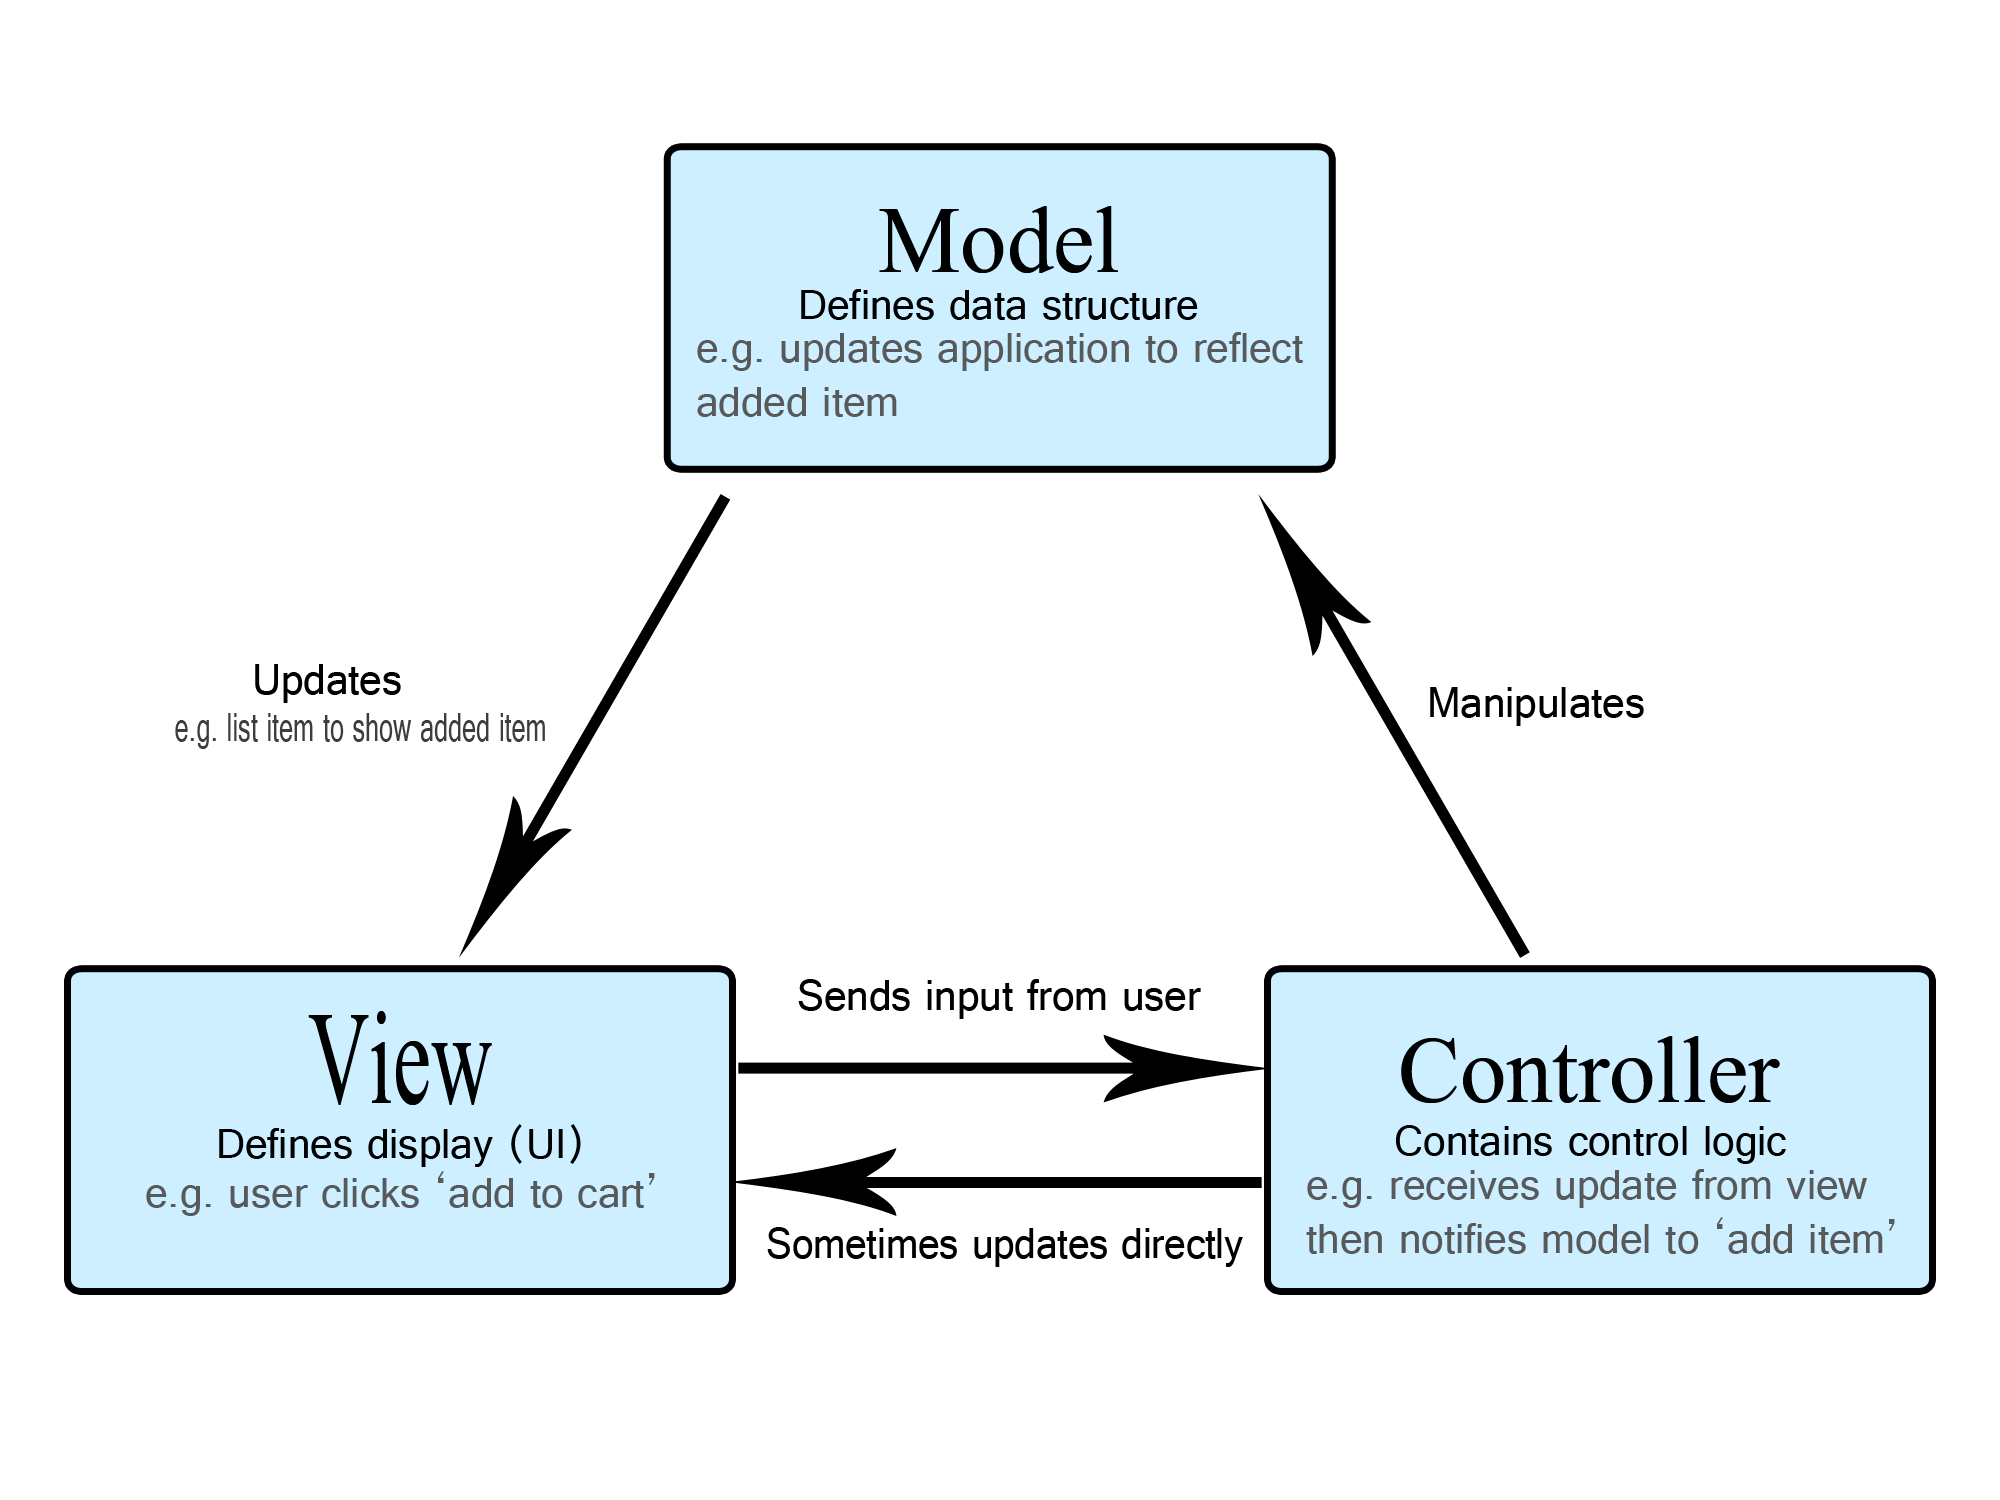
\includegraphics[scale=0.8]{graphics/model-view-controller-light-blue.png}
			\caption{MVC pattern design \cite{mvc}}
			\label{fig:MVC}
	\end{figure}
    
    
    When it comes to designing the application, as a backend developer, I focus on 5 main components below:

    \begin{enumerate}
        \item \textbf{Modular Organization:} Flask blueprints allow the application to be divided into modular components, each representing a distinct feature or functionality. I designed Blueprints to facilitate organized code by grouping related routes, templates, and static files. They are essential for large applications, promoting code reuse and separation of concerns.

        \item \textbf{URL Mapping:} Routes define the URL patterns that the application responds to and associate them with specific controller functions. Flask uses the \textbf{@app.route} decorator together with the corresponding Blueprint to map URLs to view functions. I defined all routes (corresponding to specific endpoints) of the web application, they process requests and generate appropriate responses (Rest API).

        \item \textbf{Logic Implementation:} Controllers contain the core logic for handling requests, interacting with models, and preparing data for views. They validate input, execute business logic, and orchestrate the data flow between models and views. By centralizing the application's logic, controllers ensure a clear separation of concerns.

        \item \textbf{Data Representation:} Models represent 

        \item \textbf{Reusable Components:} Common shared functions include utility functions, helper methods, and services that are used across multiple parts of the application (file utilities, database utilities, etc.). These functions promote code reuse and reduce redundancy. I organized common shared functions into separate packages named \textbf{common/}, which can be imported wherever needed. 
    \end{enumerate}

   My tasks included implementing the API endpoints, encompassing routes, controllers, and models, which provided the necessary data for the frontend. These APIs featured several critical functionalities essential for the web application. Firstly, they facilitated the upload and import of Excel billing files, ensuring seamless data integration. Secondly, the APIs enabled the visualization of billing information, presenting data in an accessible and user-friendly manner. Additionally, they provided robust filtering options to allow users to efficiently search and sort billing information. Another key feature was the generation of report charts, offering graphical representations of billing data for better insights. Lastly, the APIs supported exporting reports, allowing users to download and utilize billing information in various formats for further analysis and record-keeping.

    \subsubsection{Challenges}
    Throughout the web application development, I encountered various challenges that necessitated significant time investment in resolving them, thereby enhancing my technical proficiency.

    \begin{enumerate}
        \item \textbf{Requirement changes: } During the development phase, the requirements for the end-user interfaces and various features have changed. These changes in requirements significantly impacts the scope, timeline, and direction of the project. \\ 
        % Developers must be prepared to handle these changes efficiently and effectively.
        \textbf{\underline{Solution:}} Our team works with stakeholders to prioritize changes based on their impact and feasibility. This helps in focusing on high-value features and prevents the project from becoming overwhelming. Effective scope management ensures that critical requirements are addressed first, while less important changes can be scheduled for later.
        
        \item \textbf{Primary key constraints size limitation:} In the context of database development, the challenge arose from constraints on the size of primary keys imposed by the MySQL DBMS. \\ 
        \textbf{\underline{Solution:}} Consequently, a reassessment of the size allocation for each attribute across database entities became necessary.

        \item \textbf{Concurrency issues:} Another challenge involved concurrency issues arising from simultaneous attempts by users to upload billing excel files while other upload processes were ongoing. Resolving these issues necessitated establishing communication and coordination between these processes. \\ 
        \textbf{\underline{Solution:}} To address this, I implemented a solution using shared files. When an upload process initiates, it creates a file named \textbf{upload\_running}. Upon completion of the upload process, this file is subsequently removed. Therefore, subsequent upload processes are designed to first check for the existence of this file in the system, determining their execution based on its presence or absence.


        \item \textbf{Training for new members:} As a backend developer working on the web application project, introducing new features often necessitates bringing new team members on board to meet deadlines and ensure timely delivery. I had to ensure that new members quickly acquired the necessary knowledge about the project’s architecture, existing features, and coding standards. \\ 
        \textbf{\underline{Solution:}} Creating comprehensive and up-to-date documentation is crucial. This includes detailed architecture diagrams, API documentation, coding guidelines, and setup instructions. A well-maintained knowledge base allows new developers to self-study and reference materials as needed. Additionally, I assigned small and manageable tasks that created a supportive and efficient training environment for new members.
    \end{enumerate}


    \subsubsection{Delivery documentations}
    For the web application project, I have produced two essential documents. The first document details the API specifications using Swagger, ensuring clarity and accessibility in API implementation. The second document encompasses comprehensive guidelines for project requirements, setup procedures, and development practices. These documents aim to streamline communication, facilitate seamless integration of functionalities, and provide clear, structured guidance for efficient project development and deployment.

    

\subsection{Project output}

During my ongoing involvement in the project, I have continued to receive positive feedback from my manager regarding the code structures I have implemented and the maintenance of the project's current flow. \\

\noindent The consistency and usability of the APIs across different functionalities within the project have been notable. They have facilitated seamless integration and ease of use, contributing significantly to the overall project success. Furthermore, optimizations in database query performance have resulted in enhanced efficiency, thereby improving the user experience by ensuring quicker response times and smoother data retrieval processes. \\

\noindent The positive reception and feedback received from colleagues underscore the impact of these improvements on project outcomes. Their validation serves as a testament to the effectiveness of the technical solutions implemented. Successfully integrating and deploying backend server functionalities has further solidified my contribution to the project's objectives. This achievement reflects a combination of strategic planning, meticulous implementation, and effective collaboration with team members. \\

\noindent Looking ahead, I am committed to continuing to leverage and expand upon my skills and expertise. By staying attuned to emerging technologies and industry best practices, I aim to further enhance the project's capabilities and maintain its trajectory of success. My dedication to ongoing learning and proactive problem-solving will ensure that I continue to deliver meaningful contributions and drive continuous improvement in future endeavors.


\section{Internship Result}

\subsection{Internship target and expectation}

During my internship at BGSW Vietnam, my primary target was to bridge the gap between theoretical knowledge and practical application in the realm of web application development. I aimed to gain hands-on experience with industry-standard tools and technologies, such as Python, Flask, SQLAlchemy, and front-end frameworks. My expectations included enhancing my programming skills, understanding the full software development lifecycle, and learning to collaborate effectively within a team environment. Additionally, I sought to develop strong problem-solving abilities by tackling real-world challenges and to understand the best practices for code quality, testing, and deployment. I also anticipated gaining insights into agile methodologies and improving my ability to manage tasks and timelines efficiently. Overall, my goal was to emerge from this internship with a solid foundation in web application development and a clear understanding of the dynamics of working in a professional software development setting.

\subsection{Internship output}

Upon completing my internship at BGSW Vietnam, I have successfully achieved and exceeded my initial targets and expectations. I played a crucial role in the development of a comprehensive web application project, contributing significantly to both backend and frontend development. I developed proficiency in utilizing the Flask framework to build robust APIs, and I enhanced my skills in database management with SQLAlchemy. I also gained experience with version control using Git, and I learned how to use Docker for containerization, ensuring that our development environment was consistent and scalable. My problem-solving skills were honed as I addressed various technical challenges, such as optimizing database queries and handling concurrency issues. The internship also provided me with valuable experience in writing documentation, including API documentation with Swagger and setup guides for deployment. The positive feedback from my mentors and peers, along with the successful completion of project milestones, indicates that I have made a substantial contribution to the team. This experience has significantly boosted my confidence in my technical and collaborative abilities.

\subsection{Future path}
My immediate goal is to secure a software developer position where I can continue to refine my skills and contribute to impactful projects. I am particularly interested in roles that involve web application development, cloud computing, and data management, as these areas align with the expertise I developed during my internship. In the long term, I aspire to become a full-stack developer, capable of designing and implementing complex applications from front-end to back-end. I plan to pursue continuous learning through professional development courses, certifications, and staying updated with emerging technologies and industry trends. Additionally, I am motivated to contribute to open-source projects and participate in tech communities to broaden my knowledge and network. Ultimately, I aim to leverage my skills to create innovative solutions that address real-world problems, drive business success, and enhance user experiences.





\section{Conclusion}

This report presents the outcomes of the internship program undertaken at BGSW Vietnam, selected to fulfill the practical training requirements as an IT Developer. Throughout the internship duration, active involvement in technical skills training and engagement in the web application project constituted significant aspects of the experience. This comprehensive training encompassed various facets of software development, from backend and frontend programming to database design and system integration, providing a holistic view of the development lifecycle. \\

\noindent Engagement in the web application project was particularly enriching. It allowed for the application of theoretical knowledge to real-world scenarios, enhancing my problem-solving abilities and technical proficiency. Working on tasks such as designing database schemas, implementing API endpoints, and optimizing query performance offered practical insights into the complexities of software development. The collaborative environment at BGSW Vietnam further augmented my learning, as I received constructive feedback from mentors and collaborated with team members, fostering an atmosphere of continuous improvement. \\

\noindent The amalgamation of these factors facilitated a rich and rewarding experience within the scope of the internship program. The skills and knowledge acquired during this period have significantly bolstered my readiness to tackle professional challenges in the software development field. The internship at BGSW Vietnam has not only solidified my technical foundation but also instilled a sense of confidence and preparedness to contribute effectively to future projects. As I move forward, the experiences and lessons learned during this internship will undoubtedly serve as a cornerstone for my career development, guiding me in my journey as an aspiring software developer.
\section{Appendix}

% % citation - references
\bibliographystyle{plainurl}
\bibliography{refs.bib}
\nocite{*}


% citation - references
% \printbibliography
% \bibliographystyle{plainurl-custom}
% \bibliography{refs.bib}
% \nocite{*}


\end{document}